\documentclass[12pt, letterpaper, landscape]{article}
\usepackage[left=2cm, right=2cm, top=2cm, bottom=2cm]{geometry}
%
\usepackage{amsmath}
\usepackage{amssymb}
\usepackage{psfrag}
%\usepackage{subfig}
\usepackage[dvips]{graphicx}
%
%\newcommand{\diff}{\mathrm{d}}
%
\begin{document}
\pagestyle{empty}
\begin{figure}
\psfrag{A}{$O(1)$}
\psfrag{B}{$O(\log n)$}
\psfrag{C}{$O(n)$}
\psfrag{D}{$O(n \log n)$}
\psfrag{E}{$O(n^2)$}
\psfrag{F}{$O(2^n)$}
\psfrag{G}{$O(n!)$}
\psfrag{0}{$0$}
\psfrag{10}{$10$}
\psfrag{20}{$20$}
\psfrag{30}{$30$}
\psfrag{40}{$40$}
\psfrag{50}{$50$}
\psfrag{60}{$60$}
\psfrag{70}{$70$}
\psfrag{80}{$80$}
\psfrag{90}{$90$}
\psfrag{100}{$100$}
\psfrag{200}{$200$}
\psfrag{300}{$300$}
\psfrag{400}{$400$}
\psfrag{500}{$500$}
\psfrag{600}{$600$}
\psfrag{700}{$700$}
\psfrag{800}{$800$}
\psfrag{900}{$900$}
\psfrag{1000}{$1000$}
\psfrag{Elements}{\large Elements}
\psfrag{Operations}{\large Operations}
\psfrag{Big-O Complexity}{\Large \bf Big-O Complexity}
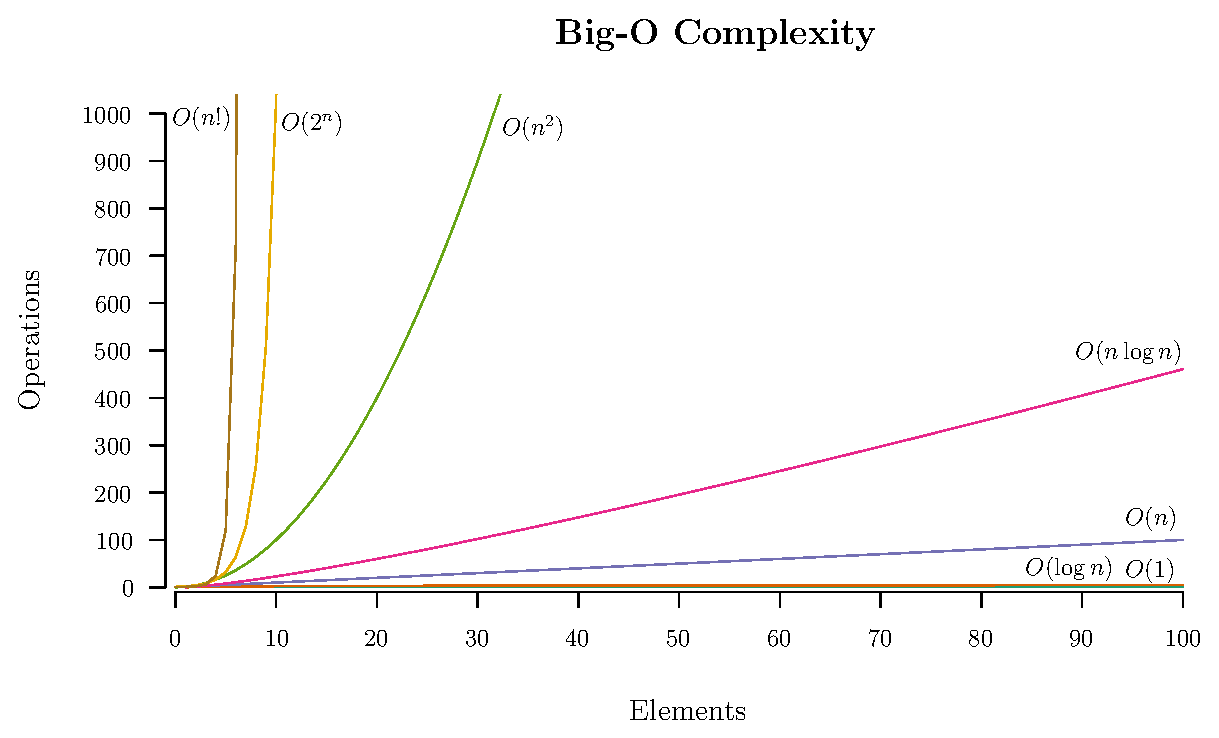
\includegraphics[scale=1]{Big-O.eps}
\end{figure}
\end{document}